\documentclass[12pt]{article}
\usepackage{amsmath}
\usepackage{tikz}
\usepackage{pgfplots}
\pgfplotsset{compat=1.17}
\usepackage{geometry}
\geometry{a4paper, margin=1in}

\title{Interest\\Couse\\
\begin{center}

\includegraphics[width=4em]{ApS_logo.png}
\end{center}
\begin{normalsize}Tutoring Centre Ferndale \end{normalsize}}
\author{}
\date{}

\begin{document}

\maketitle

\section*{Introduction}
Interest is the cost of borrowing money or the return on investment for money that is deposited or invested. There are two main types of interest: simple interest and compound interest.

\subsection*{Key Terms}
\begin{itemize}
    \item \textbf{Investment} An amount of money deposited in return for gain.
    \item \textbf{Loan} An amount of money borrowed for a price.
    \item \textbf{Principal:} The initial amount of money that is either borrowed or invested.
    \item \textbf{Interest:} The cost of borrowing money or the return earned on an investment, typically expressed as a percentage of the principal.
    \item \textbf{Rate:} The percentage of the principal charged as interest per period.
    \item \textbf{Time:} The duration for which the money is borrowed or invested, typically expressed in years.
\end{itemize}

\newpage

\section*{Simple Interest}

Simple interest is calculated on the principal amount, or on that portion of the principal amount which remains unpaid.

The formula to calculate simple interest is:
\[
I = P \times r \times t
\]
where:
\begin{itemize}
    \item \(I\) = Interest
    \item \(P\) = Principal amount (initial sum of money)
    \item \(r\) = Annual interest rate (in decimal form)
    \item \(t\) = Time (in years)
\end{itemize}

\subsection*{Example}
Suppose you invest \$1,000 at an annual interest rate of 5\% for 3 years. The interest earned would be:
\[
I = 1000 \times 0.05 \times 3 = \$150
\]

\subsection*{Exercises}

\begin{enumerate}
\item Calculate the simple interest on a principal of \$2,000 at an annual interest rate of 4\% for 5 years.
\item If you invest \$500 at an annual interest rate of 6\% for 4 years, how much interest will you earn?

\subsection*{Answers}

\setcounter{enumi}{0}
\item \(I = 2000 \times 0.04 \times 5 = \$400\)\\
\item \(I = 500 \times 0.06 \times 4 = \$120\)

\newpage

\section*{Compound Interest}

Compound interest is calculated on the initial principal, which also includes all the accumulated interest from previous periods on a deposit or loan.\\

The formula to calculate compound interest is:
\[
A = P \left(1 + \frac{r}{n}\right)^{nt}
\]
where:
\begin{itemize}
    \item \(A\) = Amount of money accumulated after \(n\) years, including interest
    \item \(P\) = Principal amount (initial sum of money)
    \item \(r\) = Annual interest rate (in decimal form)
    \item \(n\) = Number of times that interest is compounded per year
    \item \(t\) = Time (in years)
\end{itemize}\\

\subsection*{Example}
Suppose you invest \$1,000 at an annual interest rate of 5\% compounded annually for 3 years. The amount accumulated would be:
\[
A = 1000 \left(1 + \frac{0.05}{1}\right)^{1 \times 3} = 1000 \times 1.157625 = \$1157.63
\]

\subsection*{Exercises}

\setcounter{enumi}{0}
\item Calculate the amount accumulated on a principal of \$2,000 at an annual interest rate of 4\% compounded annually for 5 years.
\item If you invest \$500 at an annual interest rate of 6\% compounded quarterly for 4 years, how much will you have?

\subsection*{Answers}

\setcounter{enumi}{0}
\item \(A = 2000 \left(1 + \frac{0.04}{1}\right)^{1 \times 5} = 2000 \times 1.2166529 = \$2433.31\)
\item \(A = 500 \left(1 + \frac{0.06}{4}\right)^{4 \times 4} = 500 \times 1.2682418 = \$634.12\)

\newpage

\section*{Comparing Simple and Compound Interest}

Here are charts showing the growth of \$1,000 over 10 years with simple and compound interest at an annual rate of 5\%.

\vspace{24pt}

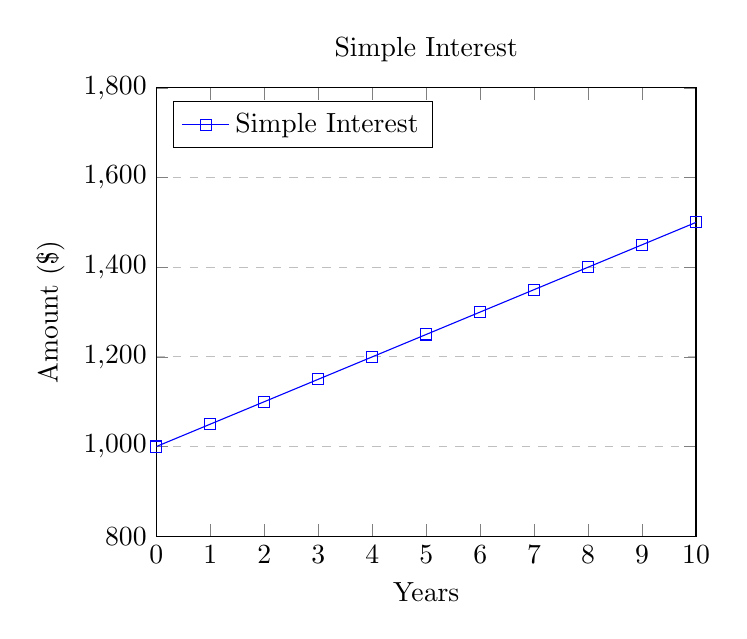
\begin{tikzpicture}
\begin{axis}[
    title={Simple Interest},
    xlabel={Years},
    ylabel={Amount (\$)},
    xmin=0, xmax=10,
    ymin=800, ymax=1800,
    xtick={0,1,2,3,4,5,6,7,8,9,10},
    ytick={800,1000,1200,1400,1600,1800},
    legend pos=north west,
    ymajorgrids=true,
    grid style=dashed,
]

\addplot[
    color=blue,
    mark=square,
    ]
    coordinates {
    (0,1000)(1,1050)(2,1100)(3,1150)(4,1200)(5,1250)(6,1300)(7,1350)(8,1400)(9,1450)(10,1500)
    };
    \legend{Simple Interest}
\end{axis}
\end{tikzpicture}

\begin{table}[ht]
\centering
\begin{tabular}{@{}c|p{2.2em}|p{2.2em}|p{2.2em}|p{2.2em}|p{2.2em}|p{2.2em}|p{2.2em}|p{2.2em}|p{2.2em}|p{2.2em}|p{2.2em}@{}}
Yr & 0 & 1 & 2 & 3 & 4 & 5 & 6 & 7 & 8 & 9 & 10\\
\hline
\$ & 1000 & 1050 & 1100 & 1150 & 1200 & 1250 & 1300 & 1350 & 1400 & 1450 & 1500\\
\end{tabular}
\end{table}

\vspace{36pt}

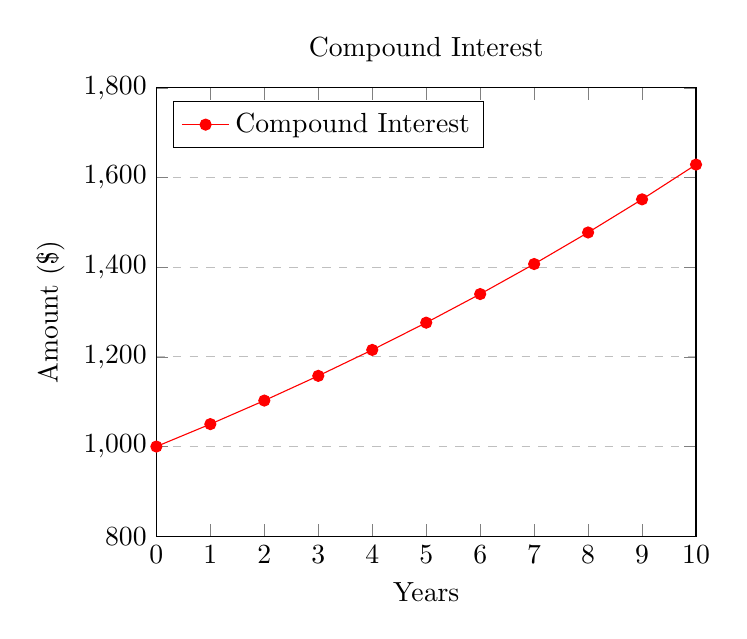
\begin{tikzpicture}
\begin{axis}[
    title={Compound Interest},
    xlabel={Years},
    ylabel={Amount (\$)},
    xmin=0, xmax=10,
    ymin=800, ymax=1800,
    xtick={0,1,2,3,4,5,6,7,8,9,10},
    ytick={800,1000,1200,1400,1600,1800},
    legend pos=north west,
    ymajorgrids=true,
    grid style=dashed,
]

\addplot[
    color=red,
    mark=*,
    ]
    coordinates {
    (0,1000)(1,1050)(2,1102.5)(3,1157.63)(4,1215.51)(5,1276.28)(6,1340.1)(7,1407.1)(8,1477.46)(9,1551.33)(10,1628.89)
    };
    \legend{Compound Interest}
\end{axis}
\end{tikzpicture}

\begin{table}[ht]
\centering
\begin{tabular}{@{}c|p{2.5em}|p{2.5em}|p{2.5em}|p{2.5em}|p{2.5em}|p{2.5em}|p{2.5em}|p{2.5em}|p{2.5em}|p{2.5em}|p{2.5em}@{}}
Yr & 0 & 1 & 2 & 3 & 4 & 5 & 6 & 7 & 8 & 9 & 10\\
\hline
\$ & 1000 & 1050 & 1102 & 1158 & 1216 & 1276 & 1340 & 1407 & 1477 & 1551 & 1629\\
\end{tabular}
\end{table}

\newpage

\section*{Examples}
\subsection*{Simple Interest}
You take out a loan of \$5,000 at a simple interest rate of 6\% per year for 4 years. How much interest will you pay and what is the total amount to be repaid?

\[
I = 5000 \times 0.06 \times 4 = \$1200
\]
The total amount to be repaid is:
\[
5000 + 1200 = \$6200
\]

\subsection*{Compound Interest}
You invest \$3,000 at an annual interest rate of 5\% compounded annually for 6 years. How much will you have at the end of the period?

\[
A = 3000 \left(1 + \frac{0.05}{1}\right)^{1 \times 6} = 3000 \times 1.3400956 = \$4020.29
\]

\newpage

\section*{Exercises}

\subsubsection*{Simple Interest}

\setcounter{enumi}{0}
\item If you borrow \$2,500 at a simple interest rate of 7\% per year for 3 years, how much interest will you pay?
\item A savings account offers a simple interest rate of 3\% per year. How much interest will you earn in 5 years on a deposit of \$1,500?

\subsubsection*{Compound Interest}

\setcounter{enumi}{0}
\item Calculate the amount accumulated on a principal of \$4,000 at an annual interest rate of 5\% compounded annually for 8 years.
\item If you invest \$1,200 at an annual interest rate of 4\% compounded semiannually for 5 years, how much will you have?

\subsection*{Answers}

\subsubsection*{Simple Interest}

\setcounter{enumi}{0}
\item \(I = 2500 \times 0.07 \times 3 = \$525\)
\item \(I = 1500 \times 0.03 \times 5 = \$225\)

\subsubsection*{Compound Interest}

\setcounter{enumi}{0}
\item \(A = 4000 \left(1 + \frac{0.05}{1}\right)^{1 \times 8} = 4000 \times 1.4774554 = \$5909.82\)
\item \(A = 1200 \left(1 + \frac{0.04}{2}\right)^{2 \times 5} = 1200 \times 1.221386 = \$1465.66\)

\end{document}
